\iffalse
\documentclass[10pt]{article}
\usepackage{graphicx}
\usepackage[none]{hyphenat}
\usepackage{graphicx}
\usepackage{listings}
\usepackage[english]{babel}
\usepackage{siunitx}
\usepackage{graphicx}
\usepackage{caption} 
\usepackage{booktabs}
\usepackage{array}
\usepackage{amssymb} % for \because
\usepackage{amsmath}   % for having text in math mode
\usepackage{extarrows} % for Row operations arrows
\usepackage{listings}
\usepackage[utf8]{inputenc}
\lstset{
  frame=single,
  breaklines=true
}
\usepackage{hyperref}
  
%Following 2 lines were added to remove the blank page at the beginning
\usepackage{atbegshi}% http://ctan.org/pkg/atbegshi
\AtBeginDocument{\AtBeginShipoutNext{\AtBeginShipoutDiscard}}


%New macro definitions
\newcommand{\mydet}[1]{\ensuremath{\begin{vmatrix}#1\end{vmatrix}}}
\providecommand{\brak}[1]{\ensuremath{\left(#1\right)}}
\newcommand{\solution}{\noindent \textbf{Solution: }}
\newcommand{\myvec}[1]{\ensuremath{\begin{pmatrix}#1\end{pmatrix}}}
\providecommand{\norm}[1]{\left\lVert#1\right\rVert}
\providecommand{\abs}[1]{\left\vert#1\right\vert}
\let\vec\mathbf{}
\begin{document}

\begin{center}
\title{\textbf{VECTORS}}
\date{\vspace{-5ex}} %Not to print date automatically
\maketitle
\end{center}

\section*{12$^{th}$ Maths - EXERCISE-10.5}

Find the position vector of a point R which divides the line joining two points  P and Q whose position vectors are P = $\myvec{2\\ 1 \\}$ and Q = $\myvec{ 1\\-3\\ }$  externally in the ratio 1:2.Also show that P is the midpoint of the linesegment RQ.

\solution

\begin{align}
\vec{P} = \myvec{ 2\\1\\} 
 \label{eq1} \\
 \vec{Q} = \myvec{ 1\\-3\\}
\end{align}
\fi
When $\vec{R}$ divides line segment joining $\vec{P}$ and $\vec{Q}$ externally,
\begin{align}
\vec{R} &= \frac{\vec{Q} -2\vec{P}}{-1} 
= \myvec{3\\5}
\end{align}
Also,
\begin{align}
\frac{ (\vec{R} + \vec{Q})}{2}
=\myvec{2\\1} =\vec{P}
\end{align}
See Fig. 
\ref{fig:chapters/12/10/5/9/Figure1}.
\begin{figure}[!h]
	\begin{center}
		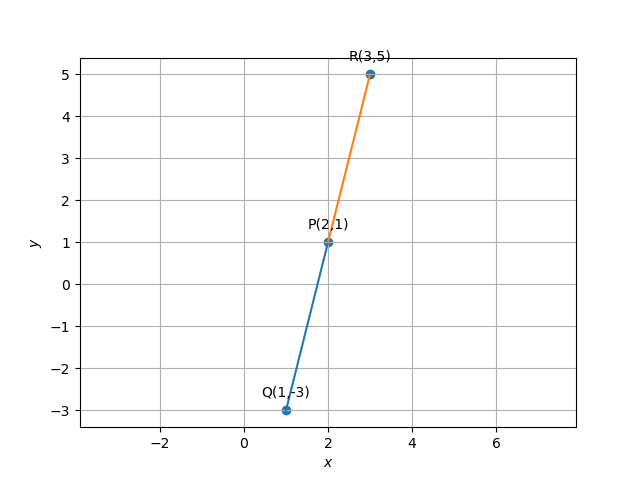
\includegraphics[width=\columnwidth]{chapters/12/10/5/9/figs/line.png}
	\end{center}
\caption{}
\label{fig:chapters/12/10/5/9/Figure1}
\end{figure}
